\documentclass[11pt,a4paper]{article}
\usepackage[margin=22mm,headheight=15pt]{geometry}
\usepackage[T1]{fontenc}
\usepackage{lmodern,microtype,graphicx,booktabs,tabularx,array,xcolor,enumitem,fancyhdr,listings,tikz,hyperref}
\usetikzlibrary{positioning,arrows.meta}
\graphicspath{{figures/}}
\definecolor{teal}{HTML}{087F74}
\definecolor{ink}{HTML}{183838}
\definecolor{pale}{HTML}{EDF6F3}
\hypersetup{colorlinks=true,linkcolor=teal,urlcolor=teal,pdftitle={Smart Maintenance Monitor -- DA3408 Project Report},pdfauthor={Sidhartha Durgam}}
\pagestyle{fancy}\fancyhf{}\fancyhead[L]{\small Smart Maintenance Monitor}\fancyhead[R]{\small DA3408}\fancyfoot[L]{\small Verified local implementation -- review copy}\fancyfoot[R]{\thepage}
\setlength{\parindent}{0pt}\setlength{\parskip}{5pt}
\setlist[itemize]{leftmargin=*,itemsep=2pt,topsep=3pt}
\setlist[enumerate]{leftmargin=*,itemsep=2pt,topsep=3pt}
\newcolumntype{Y}{>{\raggedright\arraybackslash}X}
\newcommand{\file}[1]{\path{#1}}
\newcommand{\lead}[1]{\par\vspace{4pt}\noindent\colorbox{pale}{\parbox{\dimexpr\linewidth-2\fboxsep}{\textcolor{ink}{#1}}}\par\vspace{6pt}}
\newcommand{\evidence}[2]{\begin{figure}[h!]\centering\includegraphics[width=\linewidth,height=.44\textheight,keepaspectratio]{#1}\caption{#2}\end{figure}}
\lstset{basicstyle=\ttfamily\footnotesize,breaklines=true,columns=fullflexible,frame=single,rulecolor=\color{teal},aboveskip=7pt,belowskip=7pt}
\begin{document}
\hypersetup{pageanchor=false}
\begin{titlepage}
\vspace*{12mm}
{\large\color{teal} DA3408\quad /\quad AI OPERATIONS}\par
\vspace{14mm}
{\Huge\bfseries\color{ink} Smart Maintenance\\[4pt] Monitor}\par
\vspace{7mm}
{\Large A local, reproducible machine-learning application}\par
\vspace{13mm}
\rule{\linewidth}{1pt}\par
\textbf{Prepared by}\quad Sidhartha Durgam\\
\textbf{Report date}\quad 8 November 2026\\
\textbf{Execution platform}\quad Ubuntu ARM64 virtual machine in UTM\\
\textbf{Repository}\quad \url{https://github.com/Sidhartha07D/AI-Ops-Project}
\vspace{10mm}
\lead{The project demonstrates the complete local path from pinned sensor data through Spark/Ray transformation, DVC orchestration, MLflow tracking and serving, a separate FastAPI/UI deployment, and Prometheus/Grafana monitoring.}
\textbf{Verified results}\par
13 collected unit tests passed; all 13 local CI command groups passed. A two-minute paced API measurement completed 240 requests with zero errors and a p95 of 102.46 ms. A fresh checkout restored the DVC artifacts and loaded the saved model successfully.
\vfill
\textbf{Reading this report}\par
This is a review copy of the implemented, reduced project scope. Historical results, newly measured checks, and unperformed checks are distinguished. The application classifies synthetic equipment records; it does not forecast a future failure time or guarantee industrial performance.
\end{titlepage}
\hypersetup{pageanchor=true}
\pagenumbering{roman}
\begingroup\small\setlength{\parskip}{0pt}
\tableofcontents
\endgroup
\clearpage
\pagenumbering{arabic}
\section{Problem, objectives and data}
\subsection{Problem definition}
A maintenance operator needs a simple way to inspect a machine's current sensor reading and decide whether to prioritize a human review. Smart Maintenance Monitor accepts six input fields, obtains a score from a separately served model, and displays either routine checks or an inspection recommendation.

The academic objective is an observable and reproducible application lifecycle. Model accuracy is reported to characterize the example, rather than presented as the project's principal achievement. The system runs locally within a constrained VM.
\subsection{Source and target}
The UCI AI4I 2020 Predictive Maintenance Dataset contains 10,000 synthetic records, including 339 positive \emph{Machine failure} labels. The supplied target describes failure at the observation, with no future failure horizon. The dataset is licensed CC BY 4.0; its citation and source are in Section~\ref{references}.
\par
\begin{tabularx}{\linewidth}{@{}lY@{}}\toprule
Item & Implementation \\\midrule
Inputs & Product quality type, air temperature, process temperature, rotation speed, torque, tool wear \\
Derived feature & Process temperature minus air temperature, rounded to one decimal place \\
Excluded columns & UDI and Product ID; TWF, HDF, PWF, OSF and RNF failure-mode flags \\
Fixed split & Stratified 6,000 training / 2,000 validation / 2,000 test records \\
Source integrity & Pinned raw CSV SHA-256 and schema checks before preprocessing \\\bottomrule
\end{tabularx}
\par

The failure-mode flags disclose outcomes and are excluded to prevent leakage. Preprocessing is fitted on training records only. Exact duplicate feature rows were checked and absent. Twenty-seven records whose supplied main label differs from the OR of the mode flags retain the supplied main label; the discrepancy is recorded in \file{reports/data_audit.json}.
\subsection{Data validation and identity}
The source validator checks the pinned CSV bytes, column/schema expectations, row count, labels and finite numeric values. Two independent transformations produce equivalent seven-feature tables. Raw data and model binaries are tracked through DVC; source code, parameters and metadata are tracked through Git.
\begin{lstlisting}
Raw CSV SHA-256:
dc6630cd9b1f0f853922fad78a1b6436570d3f1ec863f1dd5c4340ac56bc8a8e
Fixed split manifest SHA-256:
7a1fdd0cca26b328c176d621dd96ed62c19fa6a69ca95cb3f8ae492e781bd08a
\end{lstlisting}
\lead{The data is synthetic, not a fleet's live industrial history. There is no temporal or machine-level holdout supported by the supplied identifiers.}
\clearpage
\section{Architecture and high-level design}
\subsection{Independent blocks and interfaces}
\begin{figure}[h!]\centering
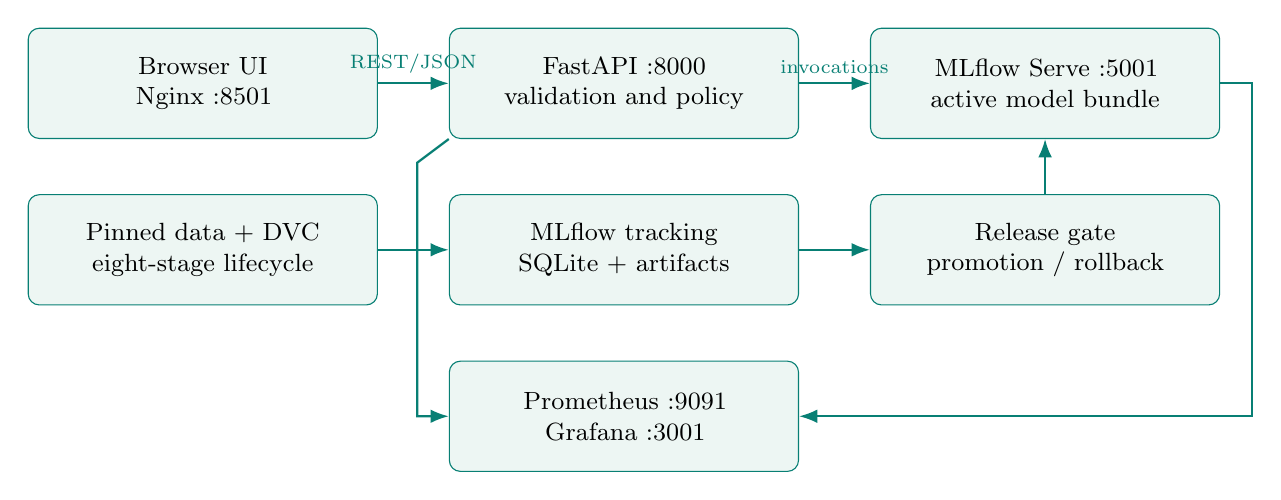
\begin{tikzpicture}[node distance=7mm and 9mm,box/.style={draw=teal,rounded corners,fill=pale,align=center,text width=42mm,minimum height=14mm,font=\small},arr/.style={-{Latex},thick,color=teal}]
\node[box](ui){Browser UI\\Nginx :8501};
\node[box,right=of ui](api){FastAPI :8000\\validation and policy};
\node[box,right=of api](model){MLflow Serve :5001\\active model bundle};
\node[box,below=of ui](dvc){Pinned data + DVC\\eight-stage lifecycle};
\node[box,right=of dvc](tracking){MLflow tracking\\SQLite + artifacts};
\node[box,right=of tracking](release){Release gate\\promotion / rollback};
\node[box,below=of tracking](monitor){Prometheus :9091\\Grafana :3001};
\draw[arr](ui)--node[above,font=\scriptsize]{REST/JSON}(api);
\draw[arr](api)--node[above,font=\scriptsize]{invocations}(model);
\draw[arr](dvc)--(tracking);\draw[arr](tracking)--(release);
\draw[arr](release)--(model);
\draw[arr](api.south west)--++(-4mm,-3mm)|-(monitor.west);\draw[arr](model.east)--++(4mm,0)|-(monitor.east);
\end{tikzpicture}
\caption{Implemented local architecture. Monitoring also includes UI and Grafana probes, node exporter and exporter self-scrapes.}
\end{figure}
The browser communicates only with FastAPI through a configurable REST base URL. FastAPI validates readings, derives the feature gap, calls the MLflow inference service and applies the active threshold. The model service owns inference. This keeps UI, application logic and model deployment separate.

Seven Compose services run concurrently: UI, API, model, Prometheus, Grafana, blackbox exporter and node exporter. Published application/monitoring ports bind to VM loopback. MLflow tracking is an on-demand host process to save RAM; its database and artifacts remain on disk.
\subsection{Design rationale}
\begin{itemize}
\item \textbf{Functional service design:} explicit preprocessing/training scripts and focused API handlers make inputs and outputs inspectable.
\item \textbf{Small deployment:} one VM, saved images, bounded Spark/Ray workers and a compact classical model fit the available resources.
\item \textbf{Reproducibility:} fixed data/split identities, DVC dependencies and clean-source candidate runs support reconstruction.
\item \textbf{Controlled deployment:} validation eligibility is separate from activation; drift never automatically promotes a model.
\end{itemize}

The API module is baked into its image under \file{/opt/smart-maintenance}; mounted \file{/workspace} supplies local data, DVC and reports. This broad workspace mount is a documented course-demo convenience rather than a least-privilege production deployment.
\clearpage
\section{Tool inventory and lifecycle orchestration}
\par
\begin{tabularx}{\linewidth}{@{}lY@{}}\toprule
Tool & Actual role \\\midrule
Git / private GitHub & Source/configuration/history; GitHub is source storage, not primary compute \\
DVC & Data/model object versioning, eight-stage DAG, local push/pull and reproduction \\
Apache Spark & Independent local CSV transformation and feature engineering \\
Ray Core & Independent parallel ETL implementation and parity comparison \\
scikit-learn / skops & Bounded classifiers, saved preprocessing/model bundles \\
MLflow & Experiment metadata, metrics/artifacts, MLproject entry points and REST model serving \\
FastAPI / Pydantic & Validated application REST API, error handling, OpenAPI \\
HTML/CSS/JavaScript / Nginx & Independent operator UI, pipeline screen, Help manual \\
Docker / Compose & Packaged model/API/UI and local monitoring services \\
Prometheus / blackbox / node exporter & Application metrics, endpoint availability and VM resources \\
Grafana & Provisioned near-real-time dashboards \\
Ruff / unittest / local CI & Formatting, selected critical lint, unit/integration/reproduction checks \\
Conda snapshot / systemd user timer & Recorded environment versions; five-minute input-drift refresh \\\bottomrule
\end{tabularx}
\par
\subsection{Eight-stage DVC DAG}
\begin{enumerate}
\item \textbf{validate\_source:} verify pinned source and write a validation record.
\item \textbf{prepare\_spark:} transform source into the canonical feature table.
\item \textbf{prepare\_ray:} independently transform the same records.
\item \textbf{compare:} check equality of row identities, values and derived features.
\item \textbf{make\_splits:} generate/reuse the fixed stratified ID manifest.
\item \textbf{train\_candidate:} fit only the 6,000 training records; record clean source/data identities.
\item \textbf{evaluate\_candidate:} score the 2,000 validation records and compute permutation importance.
\item \textbf{package\_candidate:} verify artifact identity and write a candidate release manifest.
\end{enumerate}
\subsection{Why no Airflow or Kubernetes?}
The final rubric permits Ray, Spark or Kubernetes for data engineering and names DVC for CI orchestration. This project demonstrates both Spark and Ray, with DVC managing its small file-based lifecycle. Airflow, Kubernetes/KServe and Ray Tune/Train/Serve were not added. They are explicit extensions, not claimed capabilities. Historical hosted Actions runs are retained, but automatic triggers are disabled; primary CI executes within the Ubuntu VM.
\clearpage
\section{Model development, tracking and results}
\subsection{Candidate comparison and selected policy}
Four initial baselines were compared using validation average precision (AP), suitable for the imbalanced target. The threshold was selected by validation F2 on a fixed grid, producing a threshold of 0.37.
\par
\begin{tabularx}{\linewidth}{@{}Yrr@{}}\toprule
Initial candidate & Validation AP & Recall at 0.50 \\\midrule
Prior dummy & 0.0340 & 0.0000 \\
Balanced logistic regression & 0.3679 & 0.8235 \\
Histogram gradient boosting & 0.7432 & 0.5441 \\
Balanced random forest & 0.7495 & 0.6618 \\\bottomrule
\end{tabularx}
\par

At the selected 0.37 threshold, random-forest validation recall is 0.8088. The bounded candidate configuration uses seed 42, 80 trees, maximum depth 8 and minimum leaf size 3. The UI displays an \emph{uncalibrated model failure score}; it must not be read as a calibrated field failure probability.
\par
\begin{tabularx}{\linewidth}{@{}Yrr@{}}\toprule
Selected original model & Validation & Historical test \\\midrule
Average precision & 0.7495 & 0.8066 \\
ROC AUC & 0.9768 & 0.9692 \\
Recall at 0.37 & 0.8088 & 0.8529 \\
Precision at 0.37 & 0.4661 & 0.5000 \\
F1 at 0.37 & 0.5914 & 0.6304 \\\bottomrule
\end{tabularx}
\par

Historical test confusion counts: TN 1,874; FP 58; FN 10; TP 58. These are preserved results, not a fresh test evaluation during this review.
\subsection{Experiment lineage and explainability}
The active original run is \file{e5260d1c99b046f79795c53a4c392575}. The later clean-source candidate run \file{f3f3943f9e544acc987012bec9ff0cda} logs source SHA, data/split/artifact hashes, full estimator/configuration parameters and validation metrics. It reproduces AP 0.7495 using zero test rows; no improvement is claimed.

Three-repeat validation permutation importance reports the largest AP drops for rotation speed (0.449), torque (0.423), tool wear (0.232) and temperature gap (0.199). Correlated features can redistribute importance; these values do not establish causality.
\subsection{Historical limitations retained}
The original selected training script was uncommitted at run start. Test AP appears in a failed packaging run and the successful selected run, so a strict single-use test claim is unsupported. The new clean candidate lineage does not repair the original history. The training entry point now guards against accidental repeated frozen-test evaluation.
\clearpage
\section{Low-level design and API contracts}
\subsection{Prediction input and output}
\par
\begin{tabularx}{\linewidth}{@{}lYl@{}}\toprule
Field & Validation & Unit \\\midrule
\file{type} & L, M or H & quality class \\
\file{air_temperature_k} & 250--350 & K \\
\file{process_temperature_k} & 250--400 & K \\
\file{rotational_speed_rpm} & integer, 100--5,000 & rpm \\
\file{torque_nm} & 0--100 & Nm \\
\file{tool_wear_min} & integer, 0--300 & min \\\bottomrule
\end{tabularx}
\par
\begin{lstlisting}
POST /predict
{"type":"M","air_temperature_k":298.1,
 "process_temperature_k":308.6,"rotational_speed_rpm":1551,
 "torque_nm":42.8,"tool_wear_min":0}

HTTP 200 (ID and latency vary)
{"prediction_id":"...","failure_probability":0.0117,
 "alert":false,"recommendation":"Continue routine checks",
 "threshold":0.37,"model_run_id":"e5260d1c...", ...}
\end{lstlisting}
FastAPI derives the one-decimal temperature gap and sends seven features to MLflow \file{/invocations}. It checks model output and uses the active manifest's threshold. The response field \file{failure_probability} remains for compatibility; UI interpretation is explicitly uncalibrated.
\subsection{Other endpoints and failure semantics}
\par
\begin{tabularx}{\linewidth}{@{}lY@{}}\toprule
Endpoint & Behavior \\\midrule
\texttt{GET /health} & API/model readiness and selected run ID; body distinguishes unavailable model \\
\texttt{GET /pipeline} & DVC stages/output presence, sync, candidate evaluation and recorded local CI/jobs \\
\texttt{POST /jobs/validate} & Run source validation with a bounded timeout; real console and exit status \\
\texttt{POST /feedback} & Queue a known prediction ID for review; unknown ID returns 404 \\
\texttt{GET /metrics} & Prometheus exposition of counters, histograms, readiness and freshness \\
\texttt{GET /docs} & Generated interactive OpenAPI documentation \\\bottomrule
\end{tabularx}
\par

Invalid fields return 422; unavailable model/release switching/storage write failure returns controlled 503; invalid model JSON or score returns 502. Concurrent validation can return 409. Unexpected errors are logged and sanitized. The browser flag does not approve labels or trigger training.
\clearpage
\section{Operator interface and user manual}
\begin{enumerate}
\item Open \url{http://127.0.0.1:8501/index.html} inside Ubuntu; wait for service readiness.
\item Load \emph{Routine sample} or \emph{Inspection sample}, or enter a machine type and five sensor readings within the displayed units/ranges.
\item Select \emph{Check reading}. Read the recommendation, model score, threshold and run identity.
\item Use \emph{Flag this result for review} if human follow-up is needed. This queues the existing prediction; it does not alter the model.
\item Open \emph{Pipeline status} for DVC stages, latest candidate/CI results and the real validation console. Use \emph{Help} for guidance.
\end{enumerate}
\evidence{32_model_recovery_prediction.jpg}{Actual Ubuntu Firefox result after restoring the stopped model service. The inspection example returns a 95.0\% uncalibrated score with services ready. This is a training-set demonstration record, not new test evidence.}
\subsection{Errors and responsiveness}
Native input limits prevent out-of-range submissions; server validation independently rejects invalid requests. A 390 $\times$ 844 responsive viewport and an explicit torque-range warning were captured separately. A source-validation failure console is retained as evidence. During model outage the UI identifies the unavailable service; an inference error must not be replaced by a fabricated prediction. The user manual is available as both \file{docs/user_manual.md} and browser \file{ui/manual.html}.
\clearpage
\section{Monitoring and maintenance}
\subsection{What is observed}
Prometheus gathers API request outcomes, request latency, prediction/recommendation counts, validation-job counters, service readiness and drift freshness. Blackbox exporter checks model, UI and Grafana HTTP endpoints. Node exporter provides VM available memory and root free space. Prometheus and blackbox self-scrapes extend exporter visibility.
\evidence{30_scheduled_drift_monitoring.jpg}{Actual provisioned Grafana dashboard: API, model and UI Up; prediction/latency panels; VM resources; 394 inputs in the latest drift report and recent report age. The count has a neutral display colour.}
\subsection{Input-drift workflow}
A user-level systemd timer refreshes the drift report every five minutes while the user manager is active. The checker reads up to 500 recent successful observations and requires 50 before calculating PSI. A deliberately shifted demo fixture is labeled separately. The sample count and report-age panels make a stale or sparse report visible.

Recent observations include repeated demo and automated-test requests. Input distribution shift is not proof of concept drift or degraded labeled model quality. No delayed-label accuracy monitor is claimed. Drift can motivate a validation-only candidate, but cannot invoke automatic promotion. MLflow tracking and offline jobs are on demand; persistent job reports are not internal live process metrics.
\clearpage
\section{Testing and measured performance}
\subsection{Current automated verification}
Execution used an Ubuntu ARM64 UTM VM with four virtual CPUs and about 3.3 GiB RAM, Python 3.11.18 and Java 17. Monitoring services remained part of the local deployment.

The primary command is \texttt{python scripts/local\_ci.py}, executed in the VM. Verified implementation source: \file{b77b44db} (full SHA and logs are in the archived JSON). All 13 command groups passed; all 13 collected unit cases passed with zero failures, errors or skips. Command groups are not additional unit test cases.
\par
\begin{tabularx}{\linewidth}{@{}lY@{}}\toprule
Verification layer & Observed checks \\\midrule
Code/environment & Ruff format, selected critical lint, Python compilation; exact Python and 163 pip-version checks \\
Unit tests & Input/model contract, threshold and error paths; storage failure, feedback identity, release locks, frozen-test guard and restoration fixture \\
Data/reproducibility & DVC reproduce and local push, Spark/Ray parity, Compose configuration \\
Live integration & Model/API/UI health; routine/inspection inference; invalid input; pipeline and validation console; feedback \\
Operations & Fresh drift and recorded release-history checks; separate live promotion/rollback/recovery evidence \\\bottomrule
\end{tabularx}
\par
\subsection{Data-engineering benchmark}
One measured local run on 10,000 rows used two local workers per framework. Times include startup and CSV write.
\par
\begin{tabularx}{\linewidth}{@{}Yrr@{}}\toprule
Framework & Wall time & Rows/s \\\midrule
Spark 3.5.7 & 7.62 s & 1,312 \\
Ray 2.59.0 & 4.37 s & 2,288 \\\bottomrule
\end{tabularx}
\par
Both outputs passed row-by-row comparison and shared a SHA-256 digest. Startup dominates this small workload; the result does not establish framework scale superiority or whole-job peak memory.
\subsection{Inference measurement}
The separate two-minute run used two clients, each paced to at most one request per second: 240 requests, 240 successes, zero errors over 120.003 s. Measured p50/p95/p99 were 81.77/102.46/120.87 ms. Every response matched the saved model within $10^{-6}$. Source: \file{60168ec0}; raw report: \file{reports/sustained_load.json}.

This is the achieved latency of a specified local workload, not saturation capacity or a guaranteed SLA. It uses repeated training-set demo inputs without label scoring. The unpaced short 40-request probe has different pacing and must not be compared as a capacity regression. No model-quality result was recomputed from the frozen test set.
\clearpage
\section{Release safety, persistence and recovery}
\subsection{Gated deployment}
The release gate verifies the split manifest, schema, zero candidate test rows, artifact digest and actual loadable bundle. It recomputes validation AP and recall to reject forged metadata. Only an explicit promotion command can activate an eligible candidate.

Prediction requests hold a shared release lock; a switch holds the exclusive lock. Switching stops the model, copies the candidate, recreates/verifies the served model and atomically replaces its policy manifest. On failure it restores the original bytes and policy and restarts the original service. The switch intentionally has downtime. Multi-host atomic deployment and zero downtime are not claimed.

Actual successful promotion and rollback were executed. A separately injected exception after real candidate-server startup exercised recovery to the original model. Corrupted digest and forged-metric fixtures were rejected. If recovery itself fails, the gate raises an operator error rather than claiming success.
\subsection{Restart and independent restore}
All seven service containers were stopped/removed and recreated using Compose. Model/API/UI endpoints then returned 200, the integration smoke passed, DVC was synchronized, and the drift timer was active. The report \file{reports/service_restart_check.json} distinguishes this from a full operating-system reboot, which was subsequently performed successfully as described below.

A full Ubuntu reboot was subsequently verified by a changed boot ID. Both model digests and the active policy were preserved; all seven services restarted, live integration passed, DVC stayed synchronized, and the drift timer was active. MLflow SQLite integrity remained valid with 22 runs. See \file{reports/vm_reboot_check.json}.

A temporary clean source checkout at \file{60168ec0} used a new DVC cache/workspace and pulled artifacts from the local store. DVC status was clean; active and candidate digests matched; the restored model loaded and predicted 0.01169984 for the routine example. Exact commands are in \file{reports/current_restore_check.json}. This reused the existing Python environment; it is not a fresh environment/image installation.
\subsection{Persistence and operating procedure}
Git records source and reports. DVC's VM-local store holds data/model objects; \file{mlflow_store/} holds SQLite tracking data and artifacts. Separate Mac backups preserve a Git bundle and artifact/tracking archive. Integrity checks verified 33 DVC objects and a valid SQLite database containing 22 runs at that checkpoint.
\begin{lstlisting}
cd ~/smart-maintenance-monitor
docker compose up -d --wait
~/miniconda/envs/smart-maintenance/bin/python scripts/local_ci.py
systemctl --user status smm-drift.timer
# Before shutting down Ubuntu:
docker compose down
\end{lstlisting}
Do not retrain merely because the VM restarts. Rebuild the API image after API source changes. The declared environment snapshot checks existing versions; a fresh dependency reconstruction and offline Docker-image distribution remain unverified.
\clearpage
\section{Requirements coverage and remaining boundaries}
\par
\begin{tabularx}{\linewidth}{@{}>{\raggedright\arraybackslash}p{40mm}Y@{}}\toprule
Professor's graded area & Implemented evidence \\\midrule
UI/UX (3) & Independent form, errors, responsive proof, nontechnical manual \\
Pipeline visualization (2) & Eight DVC stages, candidate summary, local CI/job outcomes and console \\
Design (2) & Architecture/HLD, independent REST boundaries, LLD and exported OpenAPI \\
Implementation (2) & Formatted Python, logging, controlled errors, release locking \\
Testing (1) & Named plan, 13 collected unit cases, real reports and integration \\
Data engineering (2) & Independent Spark/Ray transformations and measured throughput \\
Source control/CI (2) & Git/DVC identities and DAG; primary VM-only local CI \\
Experiment tracking (2) & MLflow parameters/metrics/artifacts and clean candidate lineage \\
Monitoring (2) & Prometheus instrumentation, endpoint/host probes, Grafana and drift freshness \\
Packaging (2) & MLproject declarations, MLflow Serve, FastAPI, separate Compose blocks \\
Viva (5) & Guide prepared; personal project/Assignments 1--10 explanation is the student's task \\\bottomrule
\end{tabularx}
\par
Coverage is not a promised score. The mandatory documents are retained individually: architecture, high-level design, low-level design/OpenAPI, test plan/cases and nontechnical user manual. This report consolidates their implementation and evidence.
\subsection{Explicit boundaries}
The reduced scope does not implement role accounts, fleet replay, approved-feedback learning, full pipeline retry/cancel UI, Kubernetes/KServe, Airflow, authentication/TLS, or encrypted-storage proof. The VM is a local classroom deployment. Historical selected-model lineage and repeat test logging are disclosed in Section 4.

Before final handoff: record the required 5--10 minute demonstration; confirm instructor access to the private repository and the final archive arrangement. The report and video outline are review artifacts until those steps are completed.
\section{Sources and supporting records}\label{references}
\begin{enumerate}
\item UCI Machine Learning Repository. \emph{AI4I 2020 Predictive Maintenance Dataset} (2020), DOI \href{https://doi.org/10.24432/C5HS5C}{10.24432/C5HS5C}; CC BY 4.0.
\item Course repository: \url{https://github.com/sudarsun/DA3408}. Professor-supplied \emph{AI Application Evaluation Guideline} and \emph{AI Application Development Guidelines} define the assessed categories and local-compute constraint.
\item Project records (repository-relative):\\
\file{reports/model_evaluation.json}\\
\file{reports/pipeline_evaluation.json}\\
\file{reports/etl_benchmark.md}\\
\file{reports/submission_acceptance.md}\\
\file{reports/finishing_checks.md}\\
\file{evidence/verification/b77b44db/}.
\end{enumerate}
\clearpage
\appendix
\section{Selected lifecycle and outage evidence}
\begin{figure}[h!]\centering
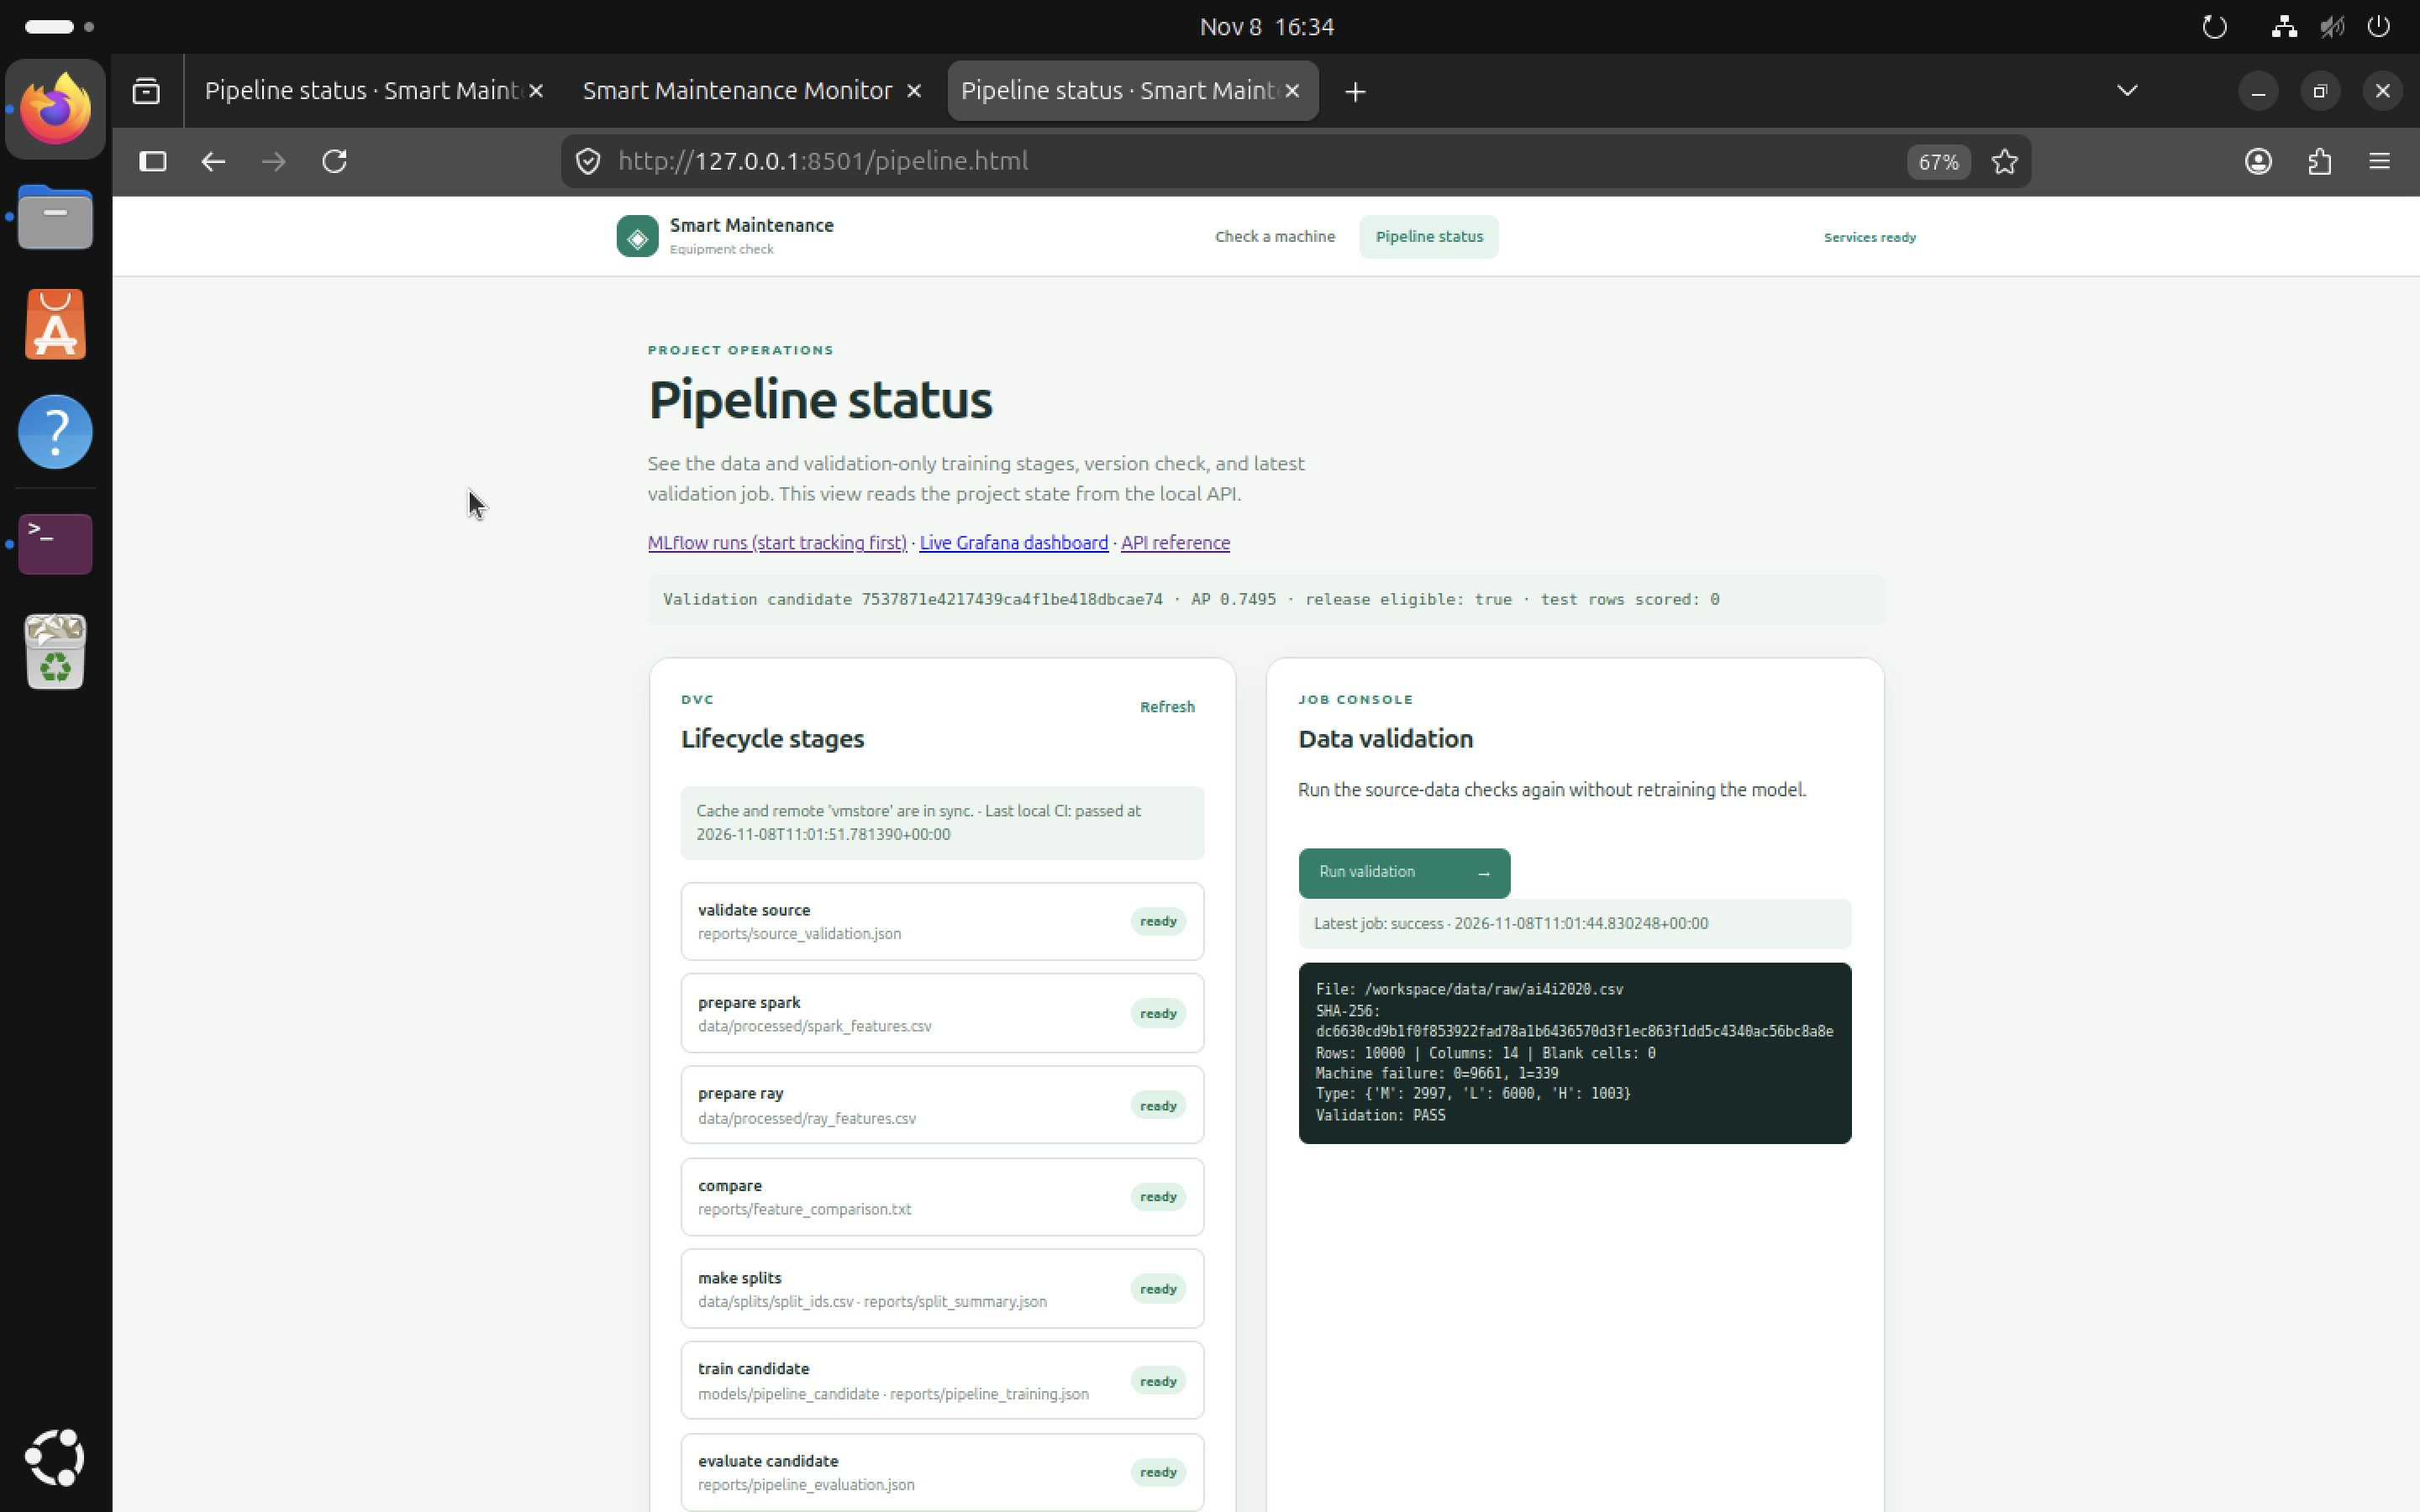
\includegraphics[width=.9\linewidth,height=.30\textheight,keepaspectratio]{29_local_lifecycle_pipeline.jpg}
\caption{Actual lifecycle screen: stage outputs, validation-only candidate lineage, local CI status and validation console. Present outputs are not a claim of newly executed cached stages.}
\vspace{5mm}
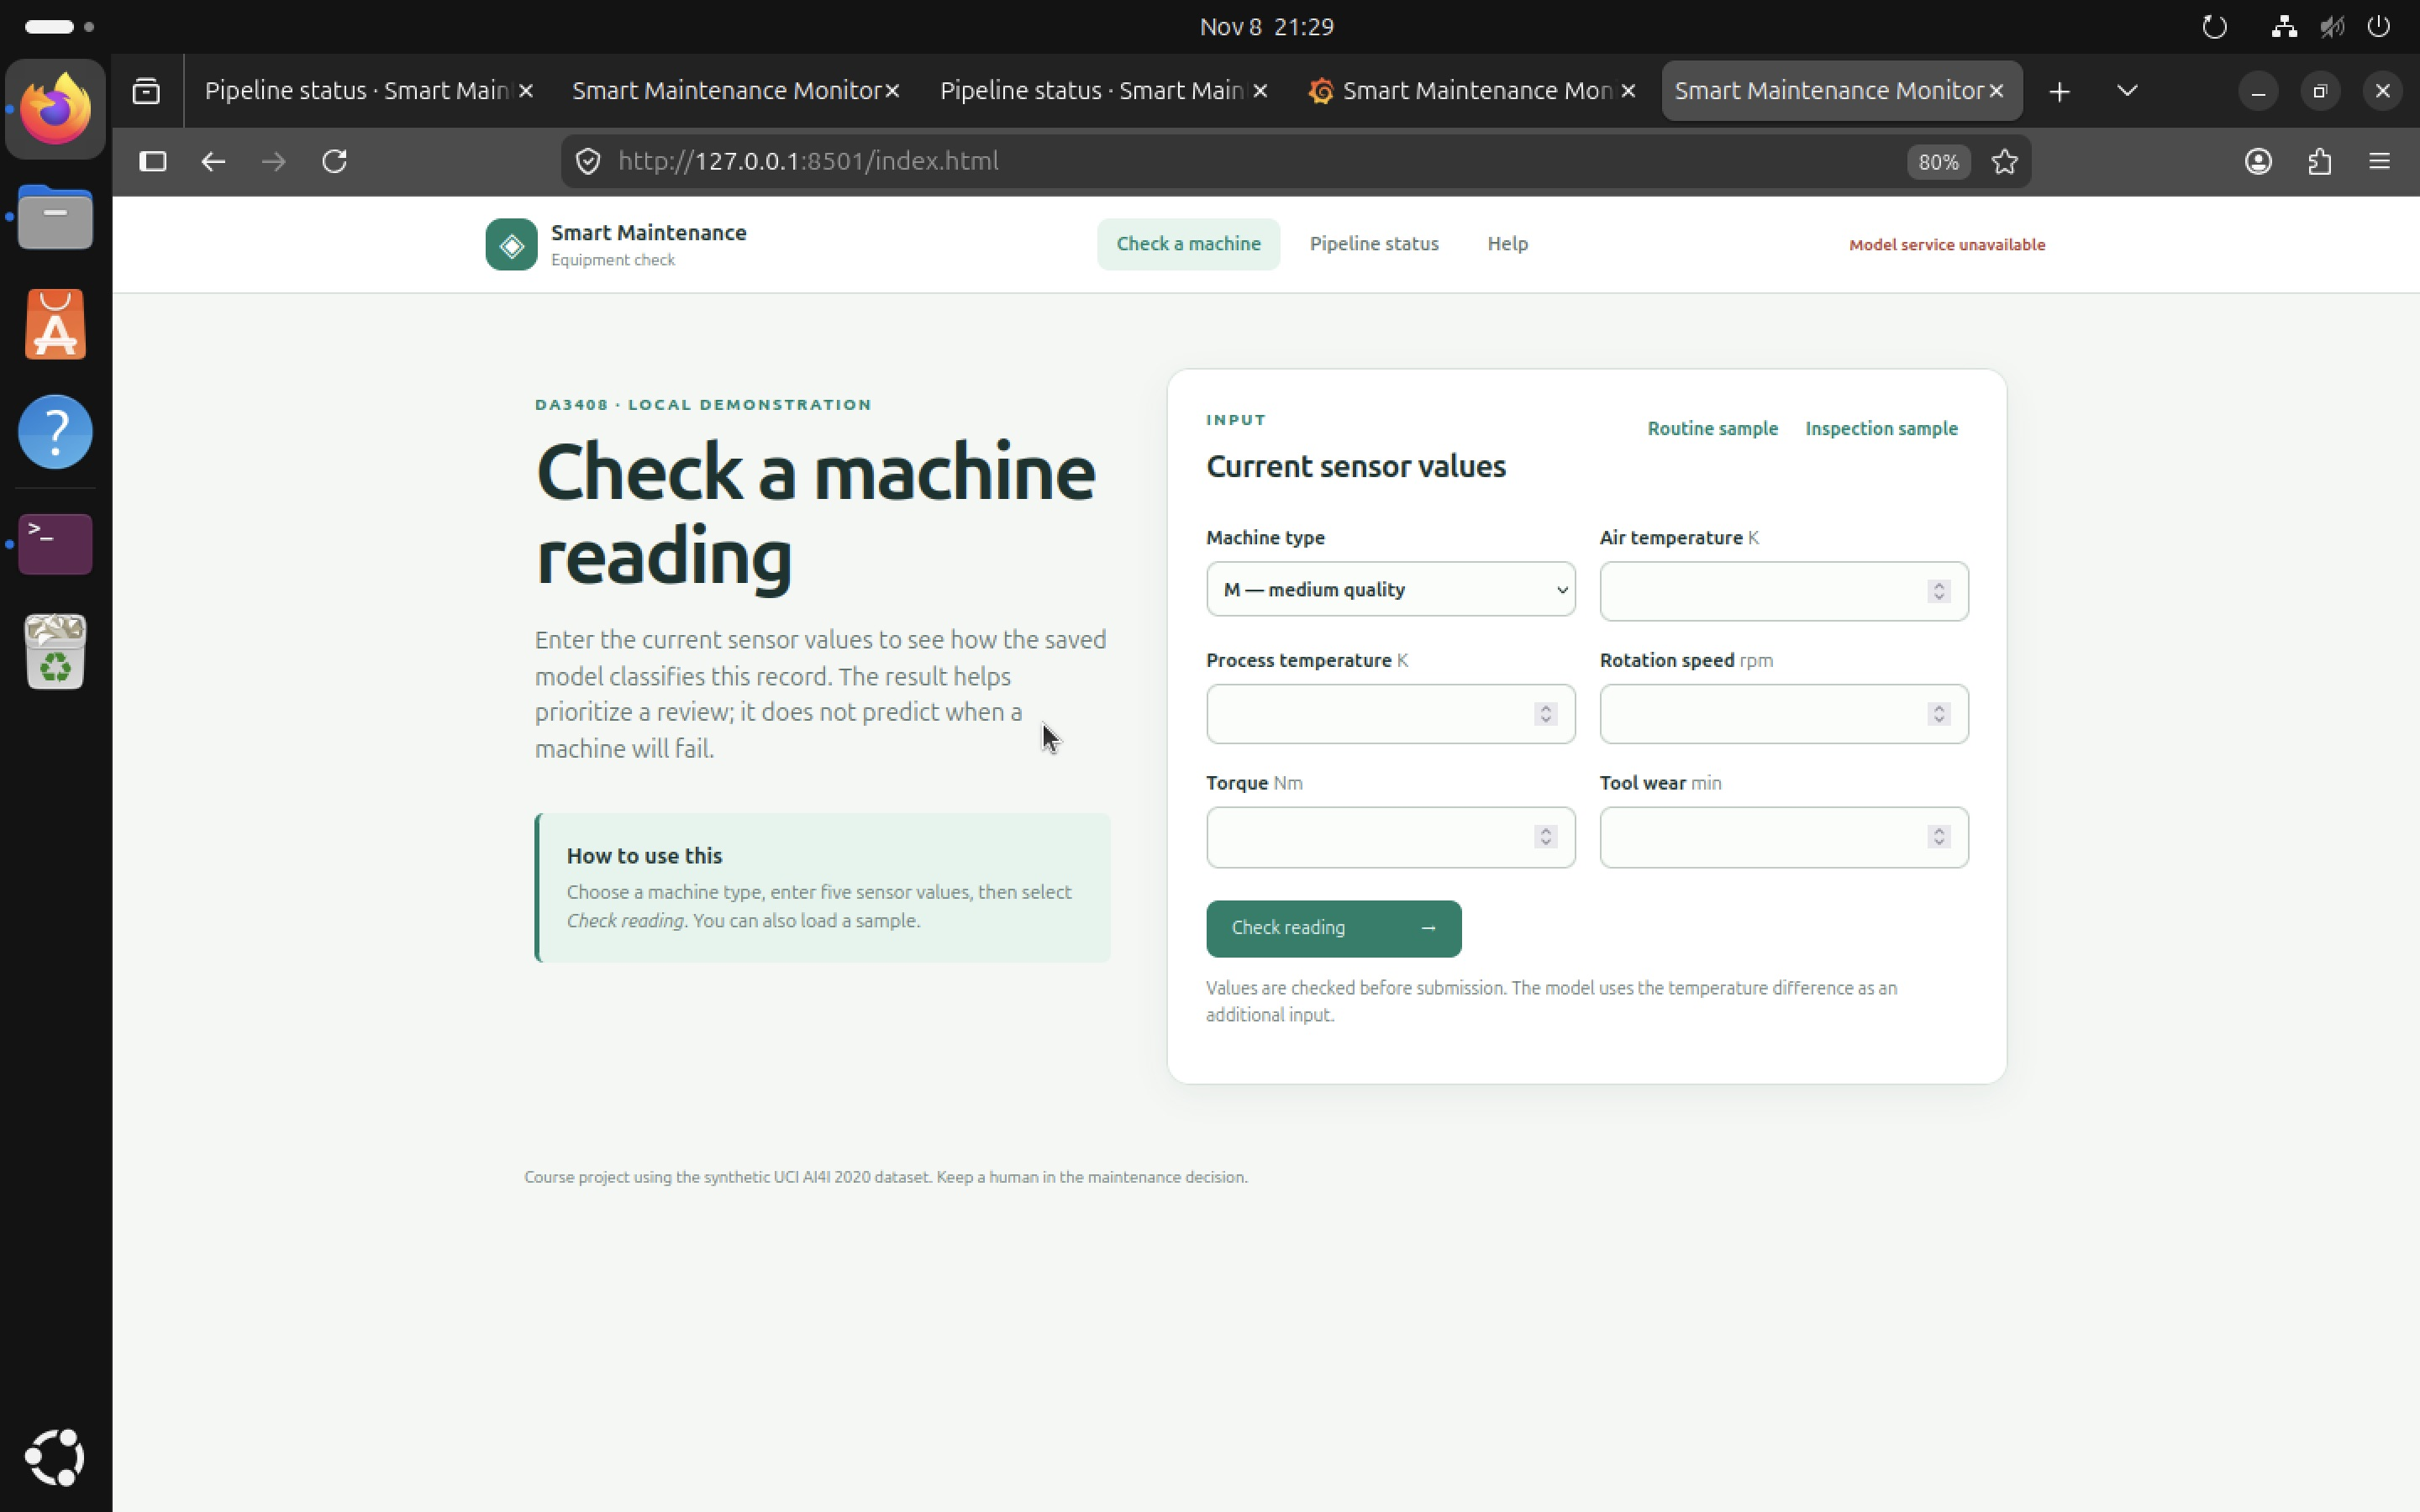
\includegraphics[width=.9\linewidth,height=.30\textheight,keepaspectratio]{31_model_outage_warning.jpg}
\caption{Genuine model outage warning while the model container was deliberately stopped. The service was restored immediately; live integration and the recovered result in Section 6 passed.}
\end{figure}
The evidence index maps each retained capture to its observed context. Mislabelled screenshot 26 was removed rather than presented as outage proof. Older redundant pipeline/Grafana views and capture tests were removed. Screenshots are actual VM captures, not generated illustrations.
\end{document}
